\documentclass{article}
\usepackage{amsmath}
\usepackage{graphicx}
\usepackage[margin=0.75in]{geometry}
\usepackage{float}
\usepackage{Sweave}
\begin{document}
\Sconcordance{concordance:eda.tex:eda.Rnw:%
1 5 1 1 0 70 1}




\section{Exploratory Data Analysis}

Our final dataset, after omitting null values, was around 2000 observations. We wanted to begin our informal analysis by plotting some data from schools with which are familiar. Therefore, we considered three cohorts - the California State University schools, the University of California schools, and the elite private schools, comprised of the Ivies and a few others. We actually considered a fourth cohort, the top-expenditure schools, but those mostly overlapped with the third cohort.



\begin{figure}[H]
\centering
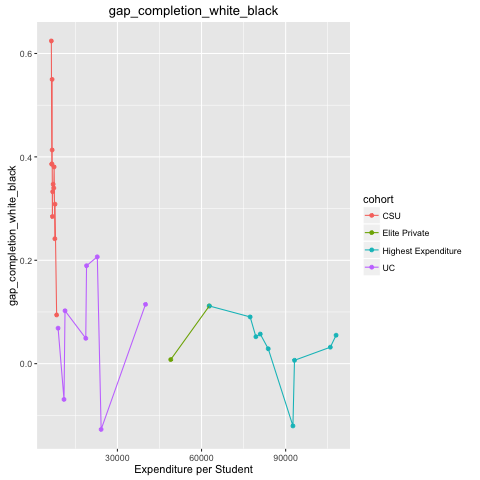
\includegraphics[width=0.3\textwidth]{../images/eda_scatterplots/gap_completion_white_black_cohort.png}
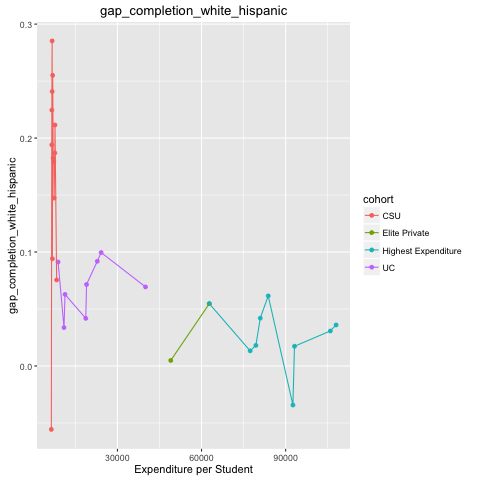
\includegraphics[width=0.3\textwidth]{../images/eda_scatterplots/gap_completion_white_hispanic_cohort.png}
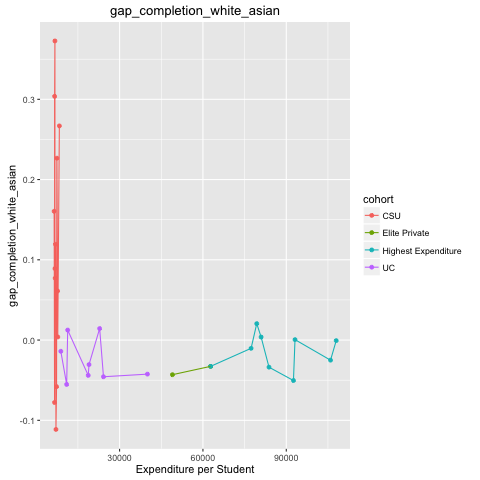
\includegraphics[width=0.3\textwidth]{../images/eda_scatterplots/gap_completion_white_asian_cohort.png}
\caption{\label{fig: CompletionRatesCohorts} We see that while there is a clear segmentation of expenditures across cohorts, the difference in outcomes is not as clear-cut. There is a general negative relationship, but a lot of variance. The most obvious conclusion is that the CSUs suffer from much worse outcome gaps than the other cohorts.}
\end{figure}

\begin{figure}[H]
\centering
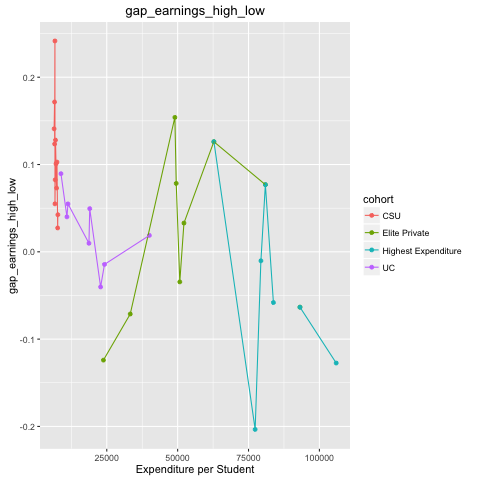
\includegraphics[width=0.3\textwidth]{../images/eda_scatterplots/gap_earnings_high_low_cohort.png}
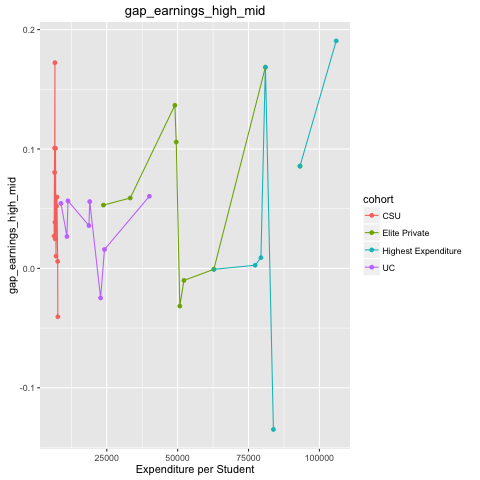
\includegraphics[width=0.3\textwidth]{../images/eda_scatterplots/gap_earnings_high_mid_cohort.png}
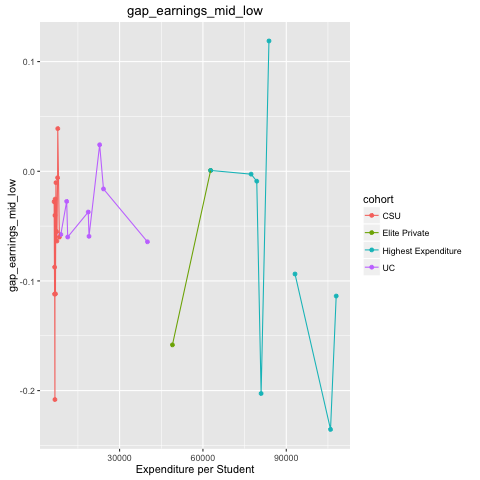
\includegraphics[width=0.3\textwidth]{../images/eda_scatterplots/gap_earnings_mid_low_cohort.png}
\caption{\label{fig:EarningsCohorts} We see a similar pattern with earnings. Interestingly, the data actually suggests that middle-income students do worse in comparison to high-income students as expenditures increase.}
\end{figure}


We now look at the full dataset to get a sense of the relationship across all schools in the US. We begin with completion rates.

\begin{figure}[H]
\centering
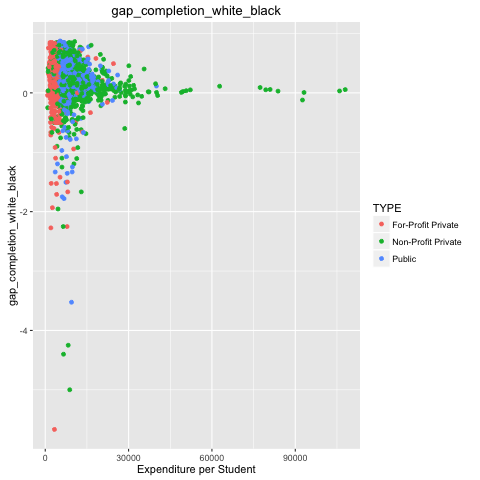
\includegraphics[width=0.3\textwidth]{../images/eda_scatterplots/gap_completion_white_black.png}
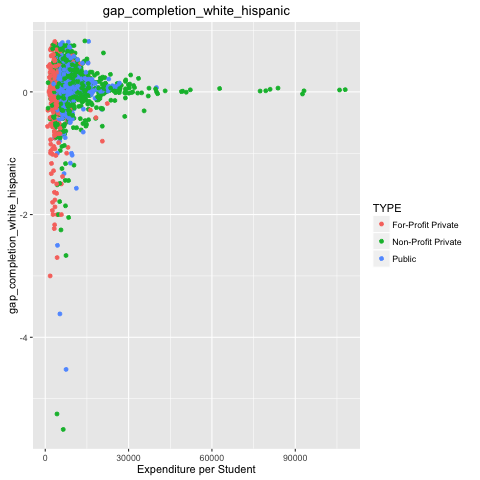
\includegraphics[width=0.3\textwidth]{../images/eda_scatterplots/gap_completion_white_hispanic.png}
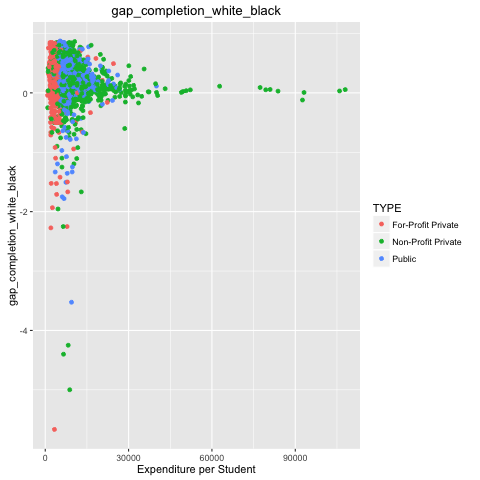
\includegraphics[width=0.3\textwidth]{../images/eda_scatterplots/gap_completion_white_black.png}
\caption{\label{fig:Completion Rates} While there are definite differences in expenditure by type of school, it is not obvious that achievement gaps decrease with expenditures. Generally, achievement gaps are not centered too far from zero, and there are quite a few outliers in both dimensions. However, it does look like variance decreases and outcome gaps cluster more closely around zero as expenditures increase.}
\end{figure}

We restrict our bounds to exclude the outliers to see if we can visually detect any patterns.

\begin{figure}[H]
\centering
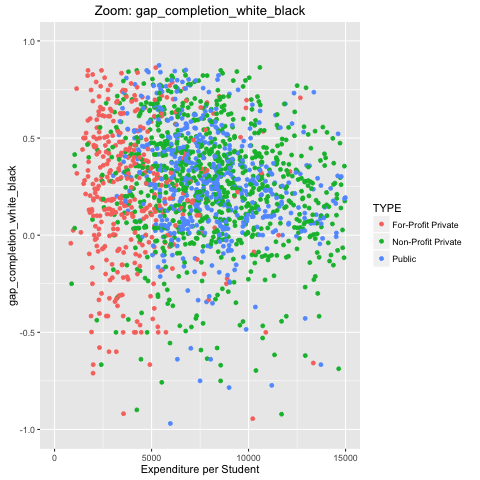
\includegraphics[width=0.3\textwidth]{../images/eda_scatterplots/gap_completion_white_black_zoom.png}
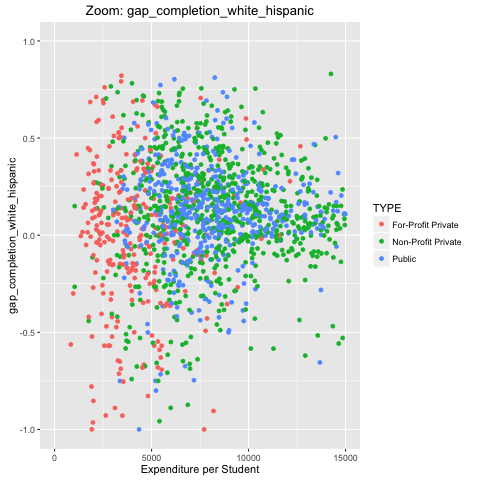
\includegraphics[width=0.3\textwidth]{../images/eda_scatterplots/gap_completion_white_hispanic_zoom.png}
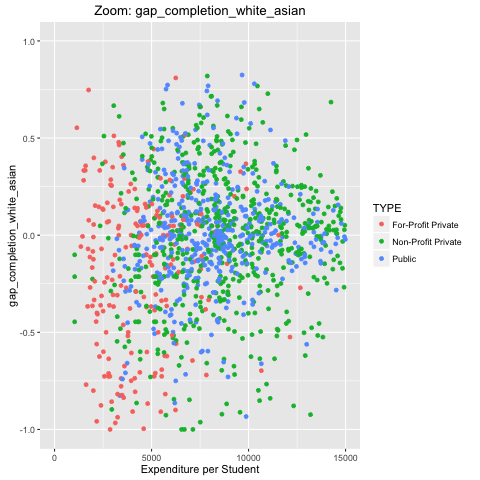
\includegraphics[width=0.3\textwidth]{../images/eda_scatterplots/gap_completion_white_asian_zoom.png}
\caption{\label{fig:Completion Rates} The data actually looks almost perfectly random.}
\end{figure}

Looking at our earnings metrics, we see a similar spread.

\begin{figure}[H]
\centering
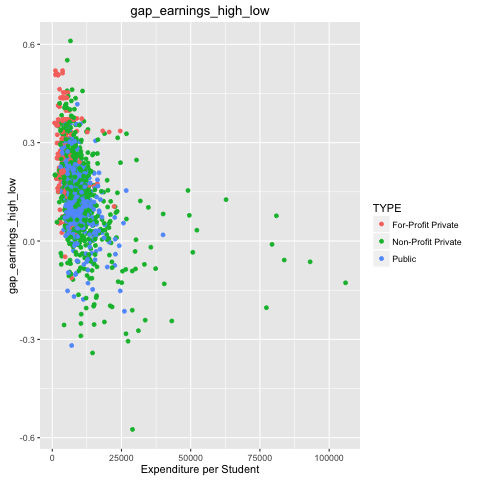
\includegraphics[width=0.3\textwidth]{../images/eda_scatterplots/gap_earnings_high_low.png}
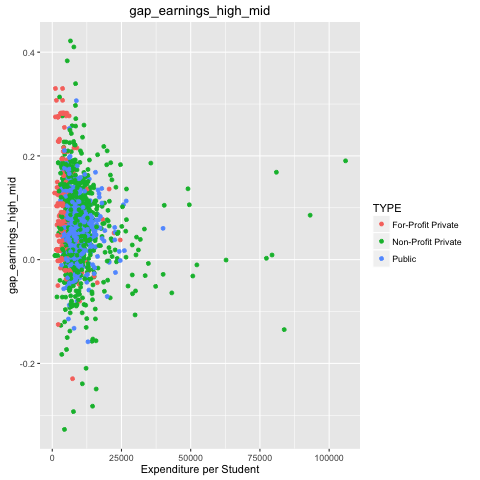
\includegraphics[width=0.3\textwidth]{../images/eda_scatterplots/gap_earnings_high_mid.png}
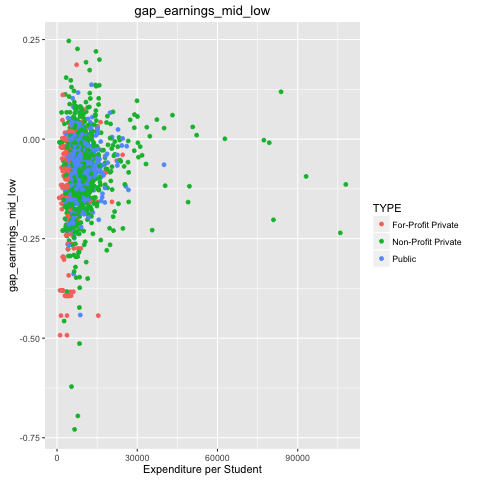
\includegraphics[width=0.3\textwidth]{../images/eda_scatterplots/gap_earnings_mid_low.png}
\caption{\label{fig:Completion Rates} We see a similar pattern, where variance decreases and the gap clusters closer to zero as expenditure increases. An interesting observation is that the gap between medium and low income terciles actually seems centered below zero - low income students on average seem to perform a bit better than their middle income peers.}
\end{figure}

However, restricting bounds produces a more interesting visual insight.

\begin{figure}[H]
\centering
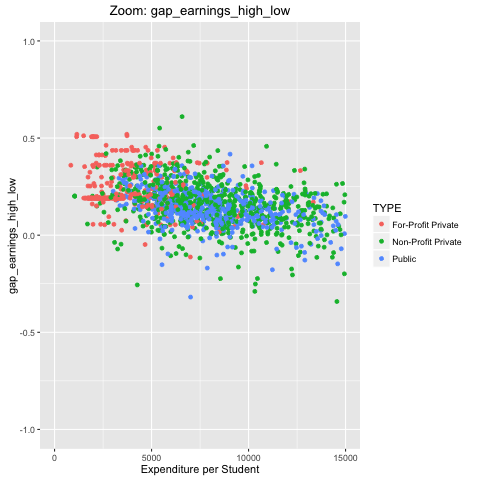
\includegraphics[width=0.3\textwidth]{../images/eda_scatterplots/gap_earnings_high_low_zoom.png}
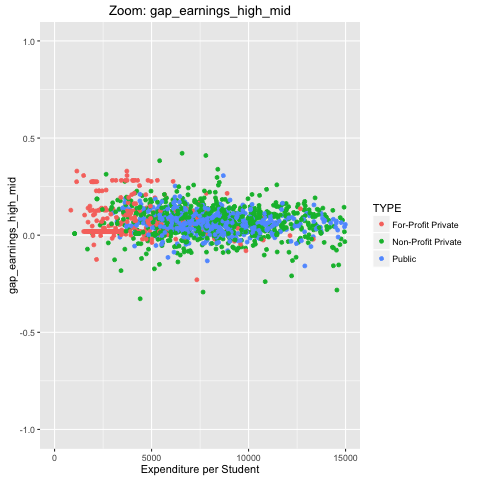
\includegraphics[width=0.3\textwidth]{../images/eda_scatterplots/gap_earnings_high_mid_zoom.png}
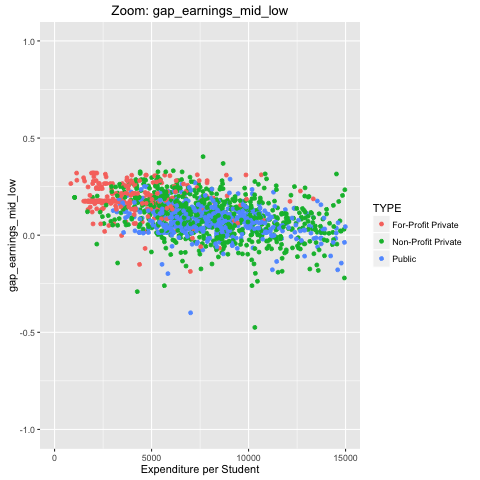
\includegraphics[width=0.3\textwidth]{../images/eda_scatterplots/gap_earnings_mid_low_zoom.png}
\caption{\label{fig:Completion Rates} Fascinatingly, we actually see a very clear negative correlation between expenditure and outcome gap for High-Low and High-Medium. Medium-Low seems to have no relationship.}
\end{figure}

The relationship between expenditure and outcome gap is not obvious, but there definitely seem to be some non-random patterns worth investigating. In the next sections, we undertake formal statistical analysis to develop more concrete conclusions about these patterns.

\end{document}
